\chapter{Introduction}

In this thesis, I want to generate a conceptual space for the domain of university courses, automatically created in data-driven way from their descriptions.

\section{Reading Instructions}

\paragraph*{Document Structure}
\todoparagraph{
	Chapter 1 is Intro, with motivations etc. 
	Chapter 2 is Background, explaining the the required concepts - what are conceptual spaces generally, how does the base algorithm work, what kinds of algorithms occur in it. I am explaining the rquired algorithm before the main algo such that I can rely on definitions there.
	Chapter 3 is then methods. Dataset, algorithm, architecture. 
	4 results, 5 conclusion, that's it.
}

\paragraph*{Terminology}

Throughout this thesis, many abbreviations, symbols and technical terms will be used. \todoparagraph{I hope that all of that cannot be exptected to be known by the reader are defined. At the end of this thesis there is a} \nameref{sec:glossary} \todoparagraph{with the subsections yadda yadda. If you are reading this document digitally, all occurrences of the terms described there should be a hyperlink (as are all section, table, figure, etc references). If you don't have the version with colored hyperlinks, you can download it here:} \url{https://nightly.link/cstenkamp/MastersThesisText/workflows/create_pdf_artifact/master/Thesis.zip}

\section{Motivation}

% ich hätte gerne sowas wie könig - mann + frau = königin \cite{Mikolov:Regularities}, nur halt mit mann und frau als einer achse

% * wie schlecht der amazon-approach wirklich ist! I mean ja, similarity-based reasoning haben sie mittlerweile sehr gut hinbekommen, aber similarity-based reasoning is the absolute basic reasoning/classification you can think of!

Dass die paar leute die in dem Bereich veröffentlichen echt aktiv sind and all und coole Ideen haben, dass die aber immer nur sich selbst zitieren (und alle auf DESC15 basieren und einen der autoren als co-author haben), und das es sinnvoll ist da mal nen sanity-check reinzubringen und als externe person die validität vom DESC15 algorithmus zu prüfen (...und dass sie ja auch alle die selben 2 datensätze nutzen und dass man eben da auch mal prüfen sollte ob deren kram so sinnvoll ist BEYOND this one dataset) - also in kurz "If this algorithm is as good as they claim, that would be great, but we have reasons to not trust their claim so we're checking them." Im Prozess dafür soll halt auch eine Pipeline rauskommen die es future research leichter macht ebengenau das zu tun was ich hier tu und die validiät der claims zu prüfen etc.

Es gibt auch arbeiten bei denen die formulierte These ein Beispiel-Anwendungsfall für die Software-Grundlage ist

in meinem Fall "Meine Ausgangsfrage war ob man die Methoden von diesem einem Paper auf educational resources anwenden kann um regelmäßigkeiten zu finden für recommendations für educational resources. Um das rauszufinden war es wichtig den Algorithmus zu entwickeln, und im verlauf der thesis ist rausgekommen das ein system dafür zu entwickeln sehr komplex ist (...dass dafür halt eine solide Software-Grundlage gegeben sein muss), also ist diese thesis primär dafür da um das system zu beshcreiben um dann mit diesem system prototypisch die fragestellung anzugehen, und die results für die originalfrage sind dann eher als priliminary results zu betrachten - fokus-shift von results zu methodik".

Das ist eine Motivation für die Thesis ganz klar ist "der Algorithmus den ich da gesehen habe ist ganz nice, das wäre doch cool wenn der so modular und reproduzierbar undundund wäre dass jemand wie ich ankommen kann und den auf andere Datensätze schmeißen kann, aber leider sind die bei open source/open data/details nennen leider nicht so super, so I'm making that instead - the delivarable is a scalable, modular, ... system that makes it easy to exchange components of it, has many analysis-scripts, etc etc etc" 
% * One of the main goals of this thesis was to create a better architecture than the shit that was available from the papers I tried to re-do here 
	% * DESC15 didn't have any code, 
	% * one of the others has a link to the repo but it's empty
	% * the last one has >40 unnamed command-line-args!)
	% * good way to bash the original paper who either didn't publish their sourcecode or link a github-repo in their paper that is fucking empty, or did at least opensource their code but have just one fucking file in there that expects >40 unnamed command-line-args

Das was ich mache ist ja eine Replikationsstudie -> Dann darf ich auch gerne diese Dinge über die Architektur undso schreiben. "Ist ja schon irgendwie ingeneurwissenschaft", dazu gehört also auch mal mehr detail wie man das gemacht hat - hängt natürlich von der gewünschten seitenzahl und dem raum den ich hab ab. In der Arbeit sollte alles drinstehen was man für die Beurteilung braucht, also quellcode oder so darf auch gerne mal im Hauptteil stehen

feature directions allow us to rank objects according to how much they have the corresponding feature, and can thus play an important role in interpretable classifiers, recommendation systems, or entity-oriented search engines, among others  [AGKS18] has many sources for these!!
	* Recommender systems (gerade critique-based ones thanks to the keyword-extraction etc)
		-> see example of [VIGSR12]
	* Semantic Search Engines (can use directions in case of gradual and possibly ill-defined features, like "popular holiday destinations")
	* Represent examples in classification tasks
	* Rule-Based Classifiers from the rankings

TODO: direkt repeatability problems ansprechen, see \url{https://cs.carleton.edu/cs_comps/1920/replication/index.php} (the paper states there is problem X, makes a claim that algorithm Y may be good at problem X, create datasets Z for X, and then test the code on these datasets. " In that test of performance, the goal is typically to identify how well the proposed algorithm works versus alternative approaches and additionally to explore what kinds of examples one's algorithm can successfully classify versus what examples it makes errors on  Future research and applications often build on these experiments, relying on their results when deciding what algorithm is most appropriate for a new task or determining whether a new algorithm is better than existing work. For instance, based on the paper above, one might conclude that to test if one has a better sarcasm detector, one need only compare against the new algorithm, since the older approach performed less well in their experiments. Yet, it's rare that people directly try to replicate other's work to confirm that the results are valid and evaluate whether the trends in the results hold in other datasets. In psychology, there has been concern in recent years that many purported psychological phenomena may be overblown, as some attempts to replicate them have been unsuccessful. While computer science experiments are not the same as psychology experiments, there is still reason to be concerned about the lack of work focused on replicating computer science experiments. Often, the details of experiments in published work are opaque, and sometimes important information for reproducing the work in not included. Replicating previous work offers the opportunity to better understand that work, and to investigate the robustness of the algorithm to changes in parameters or dataset. If the exact parameters used have major impacts on the results or the same approach on a different dataset produces very different results, it suggests that caution should be used in generalizing the results and adding nuance to the original conclusions." [quote from webpage])


Motivation of \textcite{Derrac2015} (and thus also mine, I mean I picked this bc I found what they do interesting and their idea promising): Explainable AI but data-driven (They want to get "commonsense reasoning such as interpolation and a fortiori inference", but learned automatically. As they claim, "commonsense reasoning" <=> "how different concepts and entities are semantically related" <=> CS, because "CS qualitative spatial relations" <=> "required semantic relations for reasoning"
So why do we need structured knowledge bases you ask? [Chapter 1 of DESC15]. Many CL tasks rely on structured  knowledge bases, but getting them in symbolic form occupied (computational) linguists for dozens of years without significant progress, so finding it automatically is a good idea.

\section{What are conceptual spaces? }

\cite{Derrac2015}: "Conceptual spaces \cite{Gardenfors2000} are metric spaces which are used to encode the meaning of natural language concepts and properties." %In most applications, conceptual spaces are assumed to be Euclidean. They are typically high-dimensional, with each dimension corresponding to a primitive cognitive feature. Specific entities then correspond to points in the conceptual space, while natural con- cepts and properties are posited to correspond to convex regions

% Intro of CS book: Within cognitive science, two approaches currently dominate the problem of modeling representations. The symbolic approach views cognition as computation involving symbolic manipulation. Connectionism, a special case of associationism, models associations using artificial neuron networks. Peter Gärdenfors offers his theory of conceptual representations as a bridge between the symbolic and connectionist approaches.

%TODO: mention
% * relation to prototype theory

% \cite{Derrac2015}: "Most approaches represent natural language terms as points or vectors. One notable exception is the work of G¨ardenfors on conceptual spaces [9], where properties and concepts are represented using convex regions, while specific instances of a concept are represented as points." => BUT MENTION THAT TYPES != TOKENS!!
% more DESC15: ...where properties and concepts are represented using convex regions, while specific instances of a concept are represented as points. This has a num- ber of important advantages. First, it allows us to distinguish borderline instances of a concept from more prototypical instances, by taking the view that instances which are closer to the center of a region are more typical [9]. A second advantage is that using regions makes it clear whether one concept subsumes another (e.g. every pizzeria is a restaurant), whether two concepts are mutually exclusive (e.g. no restaurant can also be a beach), or whether they are overlapping (e.g. some bars serve wine but not all, some establishments which serve wine are bars but not all). Region based models have been shown to outperform point based models in some natural language processing tasks [41] On the other hand, using regions is computationally more demanding, and learning accurate region boundaries for a given concept would require a prohibitive amount of data. In this paper, we essentially view point based representations as coarse-grained approximations of conceptual spaces, where points correspond to fine-grained categories instead of specific instances, while convex regions are used to model higher-level categories



Conceptual spaces (Gärdenfors, blabla) want to stand in between subsymbolic processing and symbolic processing: Like in subsymbolism, concepts are represented in high-dimensional spaces, but because the dimensions of these spaces are not arbitrary but human-interpretable, it allows for symbolistic high-level reasoning.

So, in conceptual spaces, concepts are represented as convex regions in high-dimensional, human interpretable spaces. For example, the concept of "apple" is a region that in the dimension "color" is somewhere between red and green, in the dimension "form" at roughly round, in the dimension "taste" somwhere between sweet and sour, etc. 
Every instance of an apple is thus a vector that lies inside the high-dimensional region of the concept. This allows for high-level reasoning, such as the question "does any Instance of concept X fit into my bag?" -> If the "size" dimension of the whole region is smaller than the size of my bag, it will.

Conceptual spaces sounds similar to \gls{word2vec} or other word embedding approaches, however there are a few important distinctions - first, the domain of a conceptual space does not include all kinds of words or concepts, but only concepts of a certain domain (like movies or university courses). 
Second, conceptual spaces are convex regions, not mere vectors (which allows for easy extraction of is-a and part-of relations or prototypical examples vs edge examples, but makes the generation computationally vastly more expensive). And, most importantly, while the geometry of \gls{word2vec} is roughly euclidian (otherwise the famous vec(king)-vec(man)+vec(woman)==vec(queen) wouldn't work), the dimensions are not interpretable but arbitrarily depend on the random initial setup, so the concepts king and queen differ not only in a single "gender" dimension [..and also its not really euclidian, is it?! sonst wäre die betweeness doch nicht so special, oder?].

Now the standard problem with conceptual spaces is that they would have to be manually generated, which of courses is a lot of work, which is where the work of [Schokeart et al] comes in - to generate them in a data-driven fashion.
For that, the authors look at three different domains: movies, wines and places. For each of these domains, they collected many samples (like movies) together with descriptions from places where people can leave them (like reviews from IMDB). A representation of a movie is then generated from the bag-of-words of the descriptions of the individual movies, leading to a very high-dimensional, very sparse representation for all movies. 
To make the representations less sparse and more meaningful, the words in the BOW are subsequently PPMI-weighted, which weights words that appear often in the description of a particular movie while being infrequent in the corpus overall higher while setting the representation of stopwords to almost zero. 
This PPMI-weighted BOW is however not yet a euclidian space yet, which is why the authors subsequently use multidimensional scaling (MDS). MDS is a diminsionality reduction technique that attempts to create a euclidian space of lower dimensionality than the original one in which the individual distances of the items are preserved as well as possible. 

With such a space, the concepts of betweeness already makes sense, but so far, the dimensions are not interpretable. So how does one automatically find such directions? In the case of movies, good dimensions may be "scariness", "funniness", "epicness", "family-friendlyness" etc. 
To find these dimensions, the authors look for these words (as well as similar words thanks to clustering) in the reviews. Then the movies are grouped into those that contain the words from the cluster often enough vs those that don't. A support-vector-machine subsquently finds a hyperplane that best divides the two groups (eg. scary and non-scary), and the orthogonal of that hyperplane is used as one axis of the new coordinate basis. 

% * Dass der tatsächliche Anwendungsbereich von CS noch sehr begrenzt ist - RaZb20 mention "they are commonly used in perceptual domains, e.g. for music cognition [Forth et al., 2010; Chella, 2015], where quality dimensions are carefully chosen to maximize how well the resulting conceptual spaces can predict human similarity judgements"
% * Dass Word Embeddings ja relativ nah an CS sind - For ex- ample, a well-known property of word embeddings is that many syntactic and semantic relationships can be captured in terms of word vector differences [Mikolov et al., 2013].
% TODO: Ist word2vec schon nen euclidian space? Why/Why not?



% \begin{figure}[H]
% 	\centering
% 	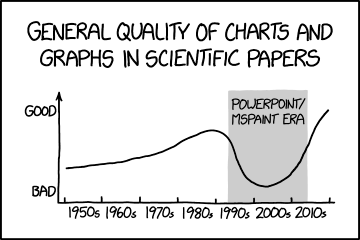
\includegraphics[width=\figwidth]{scientific_paper_graph_quality}
% 	\slcaption{
% 		Developmemt of scientific paper graph quality. A dip in the
% 		quality of scientific graphs is observed from the early 1990s to the early 2010s.
% 		During this time Microsoft Paint and PowerPoint were often used to create graphs in scientific papers.\label{fig:scientific_graph_quality}}
% \end{figure}

% \begin{table}[H]
% 	\begin{tabular}{@{}ll@{}}
% 		\toprule
% 		year & quality \\ \midrule
% 		1985 & good    \\
% 		2000 & bad     \\ \midrule
% 		2015 & better  \\ \bottomrule
% 	\end{tabular}
% 	\caption{
% 		Empirical measurements of scientific graph quality. Data points were collected using
% 		a systematic literature review.\label{tab:scientific_graph_quality}}
% \end{table}
% This references a \figref{fig:scientific_graph_quality} while this references a table \tabref{tab:scientific_graph_quality}.

% A citation looks like this \cite{hadash2018estimate}. To embed a citation in the text flow use textcite,
% \eg \textcite{hadash2018estimate} said you should use a lot of citations.

\section{What do I want to do in this thesis?}

% Ich habe schon eine eindeutige Fragestelleung ("Kann man X auf educational resources anwenden") -> danach stringent und explizit vorgehen! Das ist meine Hypothese, these are my methods, this my results, this my conclusion! 

\begin{figure}[H]
	\centering
	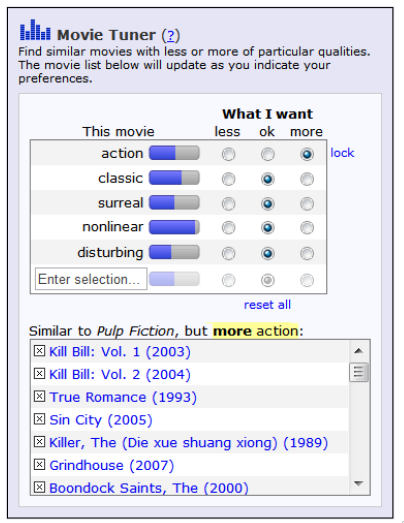
\includegraphics[width=0.7\textwidth]{graphics/stolenfigures/movietuner.png}
	\slcaption{
		The Movie-Tuner Interface from \cite{VISR12} %TODO: cite exact figure (" … as seen in [8, Fig. 33]")
		\label{fig:movetuner}}
\end{figure}

\subsection{Open Science and Reproducibility}

\label{sec:reproducibility}

% Im Snakemake-Paper https://f1000research.com/articles/10-33/v2 und auf deren startseite https://snakemake.github.io/ hauen sie einige buzzwords raus!
% Mariellas Präsi nochmal angucken
% Explainable AI!! 

from \cite{Molder2021a}: 

\begin{description}
	\item[Reproducibility] allowing validation and regeneration of results on the original or even new data. Requires understandble and well documented code.
	\item[Sustainability] such that the analysis is of lasting impact for the field, not just one research grouped
	\item[Adaptability] i.e. the ability to modify the analysis to anwer extended or slightly different research questions
	\item[Transparency] i.e. the ability for others to understand it well enough to judge if it's technically as well as methodologically valid.
	\item[Scalability] - 
\end{description}

\begin{figure}[H]
	\centering
	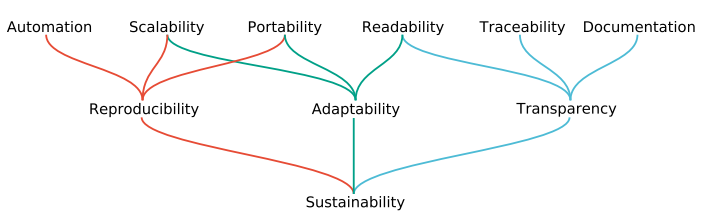
\includegraphics[width=0.7\textwidth]{graphics/stolenfigures/snakemake_aspect_hierachy.png}
	\slcaption{
		Hierarchy of aspects to consider for sustainable data analysis (reproduced from {\cite[Fig.1]{Molder2021a}}) \label{fig:snakemake_aspect_hierachy}
	}
\end{figure}


I think it is absolutely crucial for all branches of science to adhere to the principles of open science and to ensure that all claims that are made in publications are reproducible and testable. This thesis will mostly copy the work of somebody else, but doing so was incredibly tedious, much more so than it would have to be.

Dabei ist mir aufgefallen dass die schon einige DInge machen die ich aus wissenschaftlicher Sicht für ziemlich kritikwürdig halte, zum Beispiel sind die so schwammig in den Formulierungen dass man beim Versuch den Code zu reproduzieren echt viel raten muss, haben geschrieben dass der Code open ist verweisen aber auf ein leeres Repo, haben ihre Daten veröffentlicht aber wenn man damit arbeitet merkt man dass das die selbst definitiv nicht mit dem Datensatz den sie veröffentlicht haben gearbeitet haben könne, sind sehr hart am cherry-picken in ihrer qualitativ  analysis etc etc et

So one main motivation is to reproduce the code for the paper I liked in a way that adheres to the principles of open science, such that others that find it interesting don't have to go through the shit I had to go through.

Principles of open science (TODO: which are: [see thisandthis paper]) are very important to me, so I want to ensure that the claims I am making in this thesis are backed by code that is scalable, reproducible, modular, easily-understood, easily set up and run, well documented, ... . To support this, I will as often as necessary refer to the actual code in this thesis, to allow to understand and reproduce the claims and results, and also highly encourage to critically read everything here and check the respective code (...and let me know if you spot any errors! Just open a Github Issue!)

% TODO: also make the data available somewhere open!
